\documentclass{sig-alternate}
\usepackage{graphicx}
\usepackage{multiFloats}
\usepackage{url}
\usepackage{wrapfig}
\usepackage{algorithm}
\usepackage[noend]{algorithmic}
\usepackage{eqparbox}
\usepackage{array}
\usepackage{float}
\usepackage{listings}
\usepackage[flushleft]{threeparttable}
\usepackage{booktabs}
%\usepackage{mathtools}
%\usepackage{caption}
\usepackage{subfigure}
\usepackage{color}
%\usepackage[T1]{fontenc}
%\usepackage{pslatex}
\usepackage{natbib}
\usepackage{xcolor}
%\usepackage{amsthm}
\newcommand\todo[1]{\textcolor{red}{#1}}
\newtheorem{mydef}{Definition}[section]

\pdfpagewidth=8.5in
\pdfpageheight=11in

%\newcommand{\mal}{\tt}
%\newcommand{\sql}{\sf}
%\newcommand{\MAL}[1]{{\mal{}#1}}
%\newcommand{\SQL}[1]{{\sql{}#1}}

\renewcommand{\labelenumi}{(\arabic{enumi})}

\renewcommand{\textfraction}{0.0}
\renewcommand{\bottomfraction}{1.0}
\renewcommand{\topfraction}{1.0}
\renewcommand{\dbltopfraction}{1.0}
\renewcommand{\bibfont}{\scriptsize}
\renewcommand{\bibsep}{0.05cm}
%\setlength{\textfloatsep}{1ex plus1pt minus1pt}
%\setlength{\dbltextfloatsep}{1ex plus1pt minus1pt}
\renewcommand\algorithmiccomment[1]{%
  \hfill//\ \eqparbox{COMMENT}{#1}%
}
\newcommand\LONGCOMMENT[1]{%
  \hfill//\ \begin{minipage}[t]{\eqboxwidth{COMMENT}}#1\strut\end{minipage}%
}


%\usepackage{pslatex} 
%\linespread{0.97}

\pagestyle{empty}
\begin{document}

%\title{Adaptive Multidimensional Partitioning}
%\title{Shuffle Exchanging Clustering}
\title{Multidimensional Cracking in Main-memory Column-stores}

\numberofauthors{3}
\author{
\alignauthor Eleni Petraki\\
       \affaddr{CWI Amsterdam}\\
       \email{petraki@cwi.nl}
\alignauthor Lefteris Sidirourgos\\
       \affaddr{CWI Amsterdam}\\
       \email{lsidir@cwi.nl}
\alignauthor Martin Kersten\\
      \affaddr{CWI Amsterdam}\\
       \email{kersten@cwi.nl}
}

\maketitle

\begin{abstract}

What: adaptive (multi-dimensional) clustering

Why: unordered multi-dimensional data

Where: main-memory column-stores

%\vspace{5mm}
%\noindent
%{\bf Categories and Subject Descriptors:} 
%H.2 [DATABASE MANAGEMENT]: Physical Design - Access Methods\\
%%H.3 [INFORMATION STORAGE AND RETRIEVAL]: Content Analysis and Indexing -  Indexing methods
%
%%\vspace{1mm}
%%\noindent
%%{\bf General Terms:} Algorithms, Performance, Design
%
%%\vspace{1mm}
%\noindent
%{\bf Keywords:} Holistic Indexing, Self-organization

\end{abstract}



\section{Introduction}
\label{sec:introduction}

Multidimensional indexes are vital components in database systems that store
large amounts of high-dimensional data. In high-dimensional databases data 
analysis is often based on range search or nearest neighbor search queries. 
Multidimensional index structures can benefit such queries, by restricting
search to smaller areas.

Figure~\ref{fig:fcluster} shows an example of the multidimensional search
problem on the \texttt{Employees} table. The \texttt{Employees} table consists
of five attributes, i.e., the employee id, the monthly salary, the years
of experience, the age of each employee and the department each employee 
belongs to.
A database administrator (DBA) has identified a set of columns,
from the \texttt{Employees} relation where a
multidimensional clustering should be considered
\footnote{We assume the presence of a DBA for simplicity, although we 
will discuss other options later on the paper.}. For instance, consider
 columns age, salary and years of experience as the ones chosen by the DBA
to be clustered. Now consider a query of the following form.

\begin{flushleft}
\texttt{\textsc{select} age, salary, experience\\
\textsc{from} Employees\\
\textsc{where} age > 26 \textsc{and} age $\leq$ 30 \textsc{and}\\
salary > 22 \textsc{and}  salary $\leq$ 49 \textsc{and}\\
experience > 4 \textsc{and} experience $\leq$ 8}
\end{flushleft}

\begin{flushleft}
\texttt{\textsc{select} age, salary, experience\\
\textsc{from} Employees\\
\textsc{where} age > 24 \textsc{and} age $\leq$ 28 \textsc{and}\\
salary > 21 \textsc{and}  salary $\leq$ 56 \textsc{and}\\
experience > 2 \textsc{and} experience $\leq$ 7}
\end{flushleft}

\begin{figure}[t]
\begin{center}
\vspace*{3\baselineskip}
\includegraphics[trim=0cm 2cm 0cm 9.5cm, width=\columnwidth]{Figures/example_relation}
\caption{Multidimensional search on fully clustered data.}
\label{fig:fcluster}
\end{center}
\end{figure}

Ideally, to answer every query of this form we would like to have all the
relevant columns clustered as shown in Figure~\ref{fig:fcluster}.
On top of the clustered data we would use a structure to navigate directly
to the qualifying tuples. However, clustering is based on sorting, and thus,
it is a very expensive process.
Furthermore, clustering all data would delay the processing of the first query
if we did not have 
enough time to finish clustering before. To avoid penalizing user queries
with the big clustering overhead, we can \emph{partially} cluster the data.
A multidimensional index is used then to navigate search queries to clusters
with candidate qualifying tuples as shown in Figure~\ref{fig:pcluster}.
Finally, we scan the list of candidates
in order to find the tuples that qualify all predicates. 

\begin{figure}[t]
\begin{center}
\vspace*{3\baselineskip}
\includegraphics[trim=0cm 2cm 0cm 8.5cm, width=\columnwidth]{Figures/mcrack_relation}
\caption{Multidimensional search on partially clustered data.}
\label{fig:pcluster}
\end{center}
\end{figure}

Partial clustering is driven by the query predicates. For example, 
in Figure~\ref{fig:pcluster}, we first create two clusters based on the age
of the employees. Employees that are younger than 26 years belong to
the first cluster, while employees that are older than 26 years belong
to the second cluster. Similarly, the second crack, clusters the employees
that are older than 26 years into two new clusters; the first one that
contains employees that receive a monthly salary less than 50 hundred and
the second one that contains employees that receive more than 50 hundred per
month. After the two cracks, we have a list of candidate tuples,
which contains employees that are older than 26 with a monthly salary
less than 50 hundred. Out of the candidate list, we need to identify finally
those employees that are younger than 31 years, get a monthly salary
greater than 24 hundred and have an experience between 4 and 9 years.

In order to store the clustering information and to navigate to 
clusters with candidate tuples, we need a multidimensional index
structure, like a $kd$-tree. The $kd$-tree stores query predicates 
along with the cracking position in the nodes. Figure~\ref{fig:pkdtree}
shows the contents of the $kd$-tree after each crack in the previous
query. Later, we will
explain in detail how the $kd$-tree structure is adjusted to our
needs and we will provide the necessary definitions.

\textbf{Adaptive Multidimensional Indexing.}
We propose an adaptive indexing solution which minimizes the index 
creation time allowing users to query the data soon after its generation
and several times faster compared to state-of-the-art indexing approaches.  
As more queries are processed, the index is continuously refined and
subsequent queries enjoy better execution times. 
The concept of adaptive indexing has been studied in the context
of a single dimension in column-oriented databases.
In uni-dimensional cracking the main goal is to incrementally sort
individual arrays (i.e., columns) for point or range queries.
In this paper we extend the adaptive indexing idea to apply on multiple
dimensions. To  simultaneously index multiple attributes,
we need to introduce different techniques than unidimensional cracking.

\textbf{Contributions.} Our contributions are summarized as follows.
\begin{itemize}
  \setlength{\itemsep}{0pt}
  \setlength{\parskip}{0pt}
  \setlength{\parsep}{0pt}
\item We demonstrate the inability of state-of-the-art indexing to cope with exploratory analysis of very large multi-dimensional data collections. We show that the index creation time is a major bottleneck which becomes worse as data grows.
\item We introduce a novel adaptive clustering technique.  Adaptive clustering minimizes the data to query gap by integrating indexing actions with query processing and being able to immediately process user queries.
The index structure is continuously enriched as more data and queries arrive and only for the hot part of the data.
\item Furthermore,  we  propose adaptive clustering algorithms that automatically expand hot subtrees in the hot branches of the index to minimize querying costs.
\item Through a detailed experimental evaluation with both synthetic and diverse real-world workloads, we show that it is possible to drastically reduce the data to query time, being able to handle thousands of queries by the time that state-of-the-art multidimensional indexing (KDTree \cite{DBLP:journals/cacm/Bentley75}) techniques are still in the index creation phase.
\end{itemize}

\textbf{Paper outline.}
The rest of the paper is organized as follows.
In Section~\ref{sec:related_work} we discuss existing multidimensional index structures.
Section~\ref{sec:background} provides the necessary background for database cracking.
Section~\ref{sec:adaptive_partitioning} describes multidimensional adaptive indexing 
providing necessary definitions and discussions over the adaptive index built process 
and the multidimensional index structure we use.
Section~\ref{sec:experiments} describes a thorough experimental analysis with both 
real and synthetic workloads.
Finally, Section~\ref{sec:conclusions} concludes the paper.


\section{Background on Cracking}
\label{sec:background}


\subsection{Database cracking}
Cracking has been studied originally in the context of main-memory
column-stores as a simple adaptive indexing approach on \emph{one-dimensional}
data \cite{DBLP:conf/cidr/IdreosKM07} integrating data reorganization with query processing. 
For every dimension or column accessed in the workload a partial index is 
built incrementally during query processing.
The fix-point of one-dimensional database cracking is sorting the queried columns.


The data structures needed to support an end-to-end database 
cracking architecture are the following.
\begin{itemize}
\item A copy of the original column, namely \emph{cracker column}, which is
reorganized during query processing leaving the original column in the same
status.
\item A \emph{cracker index} to maintain the information about the indexed 
parts of the \emph{cracker column}.
\item A copy of the row ids used used as a \emph{map} for tuple reconstruction.
\end{itemize}

The first time a column $\mathtt{A}$ is accessed by a query, the system 
creates the cracker column $\mathtt{A_{CRK}}$,
and initializes the respective cracker index. Subsequent queries on
$\mathtt{A}$ incrementally build the cracker index by
reorganizing the underlying data into logical partitions using the query
predicates as pivots. The information about the values that are contained in
each partition is maintained in the cracker index, which is an $AVL$-tree. The
$AVL$-tree navigates subsequent queries to the correct partitions in order to
find the qualifying tuples. The qualifying tuples lay in a contiguous space in
memory which is returned as a result. To be able to reconstruct the original
tuples, the map with the original row ids is also maintained and reorganized
together with the cracker column.
Since the reorganization of the index is part of the select
operator, \emph{Database Cracking} can be seen as an alternative
implementation of scanning \cite{efficient_cracking}. 


Figure~\ref{fig:adaptive} shows how the data and the index is reorganized after
processing two subsequent queries. The first query requests values between $26$
and $31$. While searching attribute $\mathtt{Age}$ for the qualifying tuples,
the cracker column $\mathtt{Age_{CRK}}$ is reorganized such that values less than or equal to $26$ are gathered in the
first partition, values between $26$ and $31$ are gathered in the second
partition and values greater than or equal to $31$ are gathered in the third partition.
The second partition contains all qualifying values in contiguous memory and is
returned as the result. Thus, after processing the first query, values are
partitioned in three pieces. To answer the second query we navigate to the
first and the second partition (the third partition is entirely excluded from the
result) using the \emph{cracker index}. In order to find the qualifying tuples,
e.g., values between $24$ and $29$, values in the first and in the second 
partition are reshuffled using $24$ and $29$ respectively as pivots. The values
in partitions $2$ and $3$ are returned as a result. The more queries 
processed, the more partitions are created and thus subsequent queries have to
touch less and less data. When partitions are sorted or they reach a minimum size,
 found to be equal to half of the $L2$ cache size, then no further cracking 
actions take place.

\begin{figure}[t]
\begin{center}
\vspace*{3\baselineskip}
\includegraphics[trim=0cm 1cm 0cm 9cm, width=\columnwidth]{Figures/cracking_copy}
\caption{Database Cracking.}
\label{fig:adaptive}
\end{center}
\end{figure}

Database cracking has been shown to work for many core database architecture issues 
such as updates \cite{DBLP:conf/sigmod/IdreosKM07}, multi-selection/ projection queries \cite{DBLP:conf/sigmod/IdreosKM09}, concurrency control \cite{DBLP:journals/pvldb/GraefeHIKM12, CrackingTransactions}, partition-merge-like logic \cite{DBLP:conf/edbt/GraefeK10,DBLP:journals/pvldb/IdreosMKG11}. 
Stochastic database cracking \cite{DBLP:journals/pvldb/HalimIKY12} shows how to be robust on various query workloads.
Finally, \cite{IndexingKeys} shows how adaptive indexing can apply to key columns.


\begin{figure}[t]
\begin{center}
\vspace*{3\baselineskip}
\includegraphics[trim=0cm 1cm 0cm 9cm, width=\columnwidth]{Figures/sideways_cracking}
\caption{Sideways Cracking.}
\label{fig:sideways}
\end{center}
\end{figure}

\subsection{Sideways cracking}
Sideways cracking handles the tuple reconstruction for queries that
include selections and/or projections on multiple columns 
\cite{DBLP:conf/sigmod/IdreosKM09}, while \emph{partial sideways cracking} \cite{DBLP:conf/sigmod/IdreosKM09} 
reduces the storage overhead of sideways cracking.
Sideways cracking maintains and incrementally reorganizes the following data structures.

\begin{itemize}
\item \emph{Cracker maps} which consist of two columns that appear in the same query. 
A cracker map $\mathtt{M_{Ax}}$ is cracked only on $\mathtt{A}$.
The tuples of $\mathtt{x}$ are reorganized together with the tuples of
$\mathtt{A}$ to maintain the alignment between these two attributes.
All cracker maps that use $\mathtt{A}$ as the cracking column belong to 
\emph{map set $\mathtt{S_A}$}. 
\item A \emph{cracker index} (AVL-tree) for each cracker map $\mathtt{M_{Ax}}$ that maintains the information about $\mathtt{A}$.
\item A \emph{cracker tape} for each map set $\mathtt{S_A}$ that logs all cracks on $\mathtt{A}$.
Different cracker maps of the same map set use the cracker tape on demand to ensure alignment.
\item Bit vectors with bits set for the tuples that qualify both selection predicates of both columns of the cracker map.
A conjunction/disjunction of the bit vectors is used to produce the final result.
\end{itemize}

Figure~\ref{fig:sideways} shows how the data and the index is reorganized after
processing a query $\mathtt{Q_{1}}$, which includes a multiple selection and projection
on attributes $\mathtt{Age}$, $\mathtt{Salary}$ and $\mathtt{Experience}$.
To answer this query we need two cracker maps, i.e., $\mathtt{M_{AgeSal}}$ and $\mathtt{M_{AgeExp}}$.
Both maps are reorganized based on the selection predicate on $\mathtt{Age}$.
Tuples with $\mathtt{Age}$ value less than or equal to $26$ are gathered in the
first partition, values between $26$ and $31$ are gathered in the second
partition and values greater than or equal to $31$ are gathered in the third partition.
A cracker index for every map maintains the partitioning information.
While reorganizing $\mathtt{Age}$, $\mathtt{Salary}$ and $\mathtt{Experience}$ are reorganized too to ensure alignment.
After reorganizing $\mathtt{M_{AgeSal}}$ a bit vector has a bit set for all these tuples that qualify the selection predicates both on $\mathtt{Age}$ and $\mathtt{Salary}$.
Similarly, another bit vector has a bit set for all these tuples that qualify the selection predicates both on $\mathtt{Age}$ and $\mathtt{Experience}$.
The conjunction of the two bit vectors can be used to produce the final result.

Although sideways cracking handles queries with selections or projections on multiple attributes, it does so by reorganizing only one dimension at a time.

\section{Multidimensional Clustering}
\label{sec:adaptive_partitioning}

In this section we introduce the multidimensional database cracking 
architecture along with the necessary data structures and algorithms.

\subsection{Definitions and Notations}
\label{subsec:clustering}


A database administrator (DBA) identifies a set of $\mathtt{k}$ columns from a
relation $\mathtt{R}$ where multidimensional cracking should be 
considered\footnote{We assume the presence of a DBA for simplicity,
although we will discuss other options later on the paper.
The selection and the order of the $\mathtt{k}$ columns is orthogonal
to this work.}.
A copy is created for each one of the $\mathtt{k}$ columns.

We define a \textcolor{red}{\emph{cluster map}} as a subset $\mathtt{C^k=\{c_1,c_2,\ldots,c_k\}}$ of the copies of
$\mathtt{k}$ columns from a relation $\mathtt{R}$ with $\mathtt{n}$ rows. 
Values of $\mathtt{k}$ columns in the same position of the cluster map, belong to the same relational tuple.
A 
$\mathtt{k}$-dimensional query
\begin{center}
$\mathtt{Q^k = \{q_1,q_2,\ldots,q_k\ |\ q_i = [a_i, b_i],\ i=1,\ldots,k\}}$ 
\end{center}
over $\mathtt{C^k}$ returns all rows $\mathtt{r_j}$ such that
\begin{center}
$\mathtt{r_j = \{v_{j_i}\ |\ v_{j_i} \in q_i,\ i=1,\ldots,k\}}$
\end{center}
where $\mathtt{1 \leq j \leq n}$ and $\mathtt{v_{j_i}}$ is the $\mathtt{j}$-th value of $\mathtt{c_i}$
\footnote{For simplicity, we assume that a multidimensional query includes double range predicates on all $\mathtt{k}$ dimensions.
We will relax this restriction later on the paper, showing how we can handle queries with different types of predicates on a subset of $\mathtt{k}$ attributes.}.

After a cluster map is created it is used to speed up queries that access the $\mathtt{k}$ columns.
Each query triggers the physical reorganization (cracking) of the cluster map based on the query predicates.
%In the next section we describe how the reorganization of the cluster map takes place.
Here is a formal definition of multi-dimensional database cracking.

\begin{flushleft}
\begin{mydef}
Multidimensional database cracking is the clustering of 
$\mathtt{k}$ columns based on the predicates of a $\mathtt{k}$-dimensional
range query $\mathtt{Q^k}$.
\end{mydef}
\end{flushleft}



\subsection{How a query cracks a multi-dimensional partial index}
\label{subsec:mcrack}

%n-columns\\
%n-predicates*\\


%\subsection{Section To Do...}
%\label{subsec:todo}
%\textcolor{red}{There are many critical issues that we have to address in this section.
%Here is an order of their presentation.
%\begin{enumerate}
%\item What do we store in a kd-tree in adaptive clustering -> Each node stores a k-dimensional query and the first position of the ``right'' partition (split position). Define properly the k-dimensional queries.
%\item How do we insert nodes in the kd-tree.
%\item During insertion of a node(->cracking action) we need to know the limits of the to-be-cracked partition. How do we decide the limits while traversing the tree?
%\item How do we decide which partitions will be scanned/cracked/included/omitted in order to get the final row ids of the tuples that qualify the predicate.
%\item How can the kd-tree be used to answer different queries on the same dimensions (or a subset of the dimensions).
%\end{enumerate}}
%\textcolor{red}{We should also examine whether a $kd$-tree can be used for a subset of $k$ columns or not. Ideally, the same $kd$-tree should be used for any subset of the $k$ columns, where the creation of the tree was based on. For instance, if the $kd$-tree is built based on queries on $\{\mathtt{C_1,C_3,C_5,C_6}\}$, then the same $kd$-tree can be used to qualify queries just on $\{\mathtt{C_3,C_5}\}$}.

In this section we describe in detail the steps we follow to answer a multi-dimensional query $\mathtt{Q^k}$.
To answer such a query with sideways cracking, we would need $\mathtt{k-1}$ cracker maps.
The head of all cracker maps would be the same attribute.
Thus, we would need to replicate the head attribute $\mathtt{k-1}$ times.
All cracker maps are reorganized based on the head, i.e., cracking the head and reorganize the tail at the same time, to ensure alignment.
The cracker index and the cracker tape is updated with the new cracking steps on the head of the cracker maps.
In order to find the qualifying tuples of each attribute, we need to scan those tuples that qualify the head predicate and create an intermediate bit vector for every cracker map.
In the end we need to apply a conjunction on all intermediate bit vectors to retrieve the final qualifying tuples out of a contiguous piece in memory.

\begin{figure}[t]
\begin{center}
\vspace*{3\baselineskip}
\includegraphics[trim=0cm 2cm 0cm 8.5cm, width=\columnwidth]{Figures/mcrack_relation_full}
\caption{Multidimensional search on partially clustered data.}
\label{fig:mcluster_full}
\end{center}
\end{figure}

To avoid copying the head $\mathtt{k-1}$ times, we could have a cracker map that includes of all $\mathtt{k}$ attributes.
A brute-force approach would be to reorganize every column based on all respective predicates for every query and maintain this information in a proper index.
Figure~\ref{fig:mcluster_full} shows an example.
All resulting tuples lay in a contiguous area in memory (the dashed box), which we can immediately return without extra bit vector operations.
However, with this approach, for every query $\mathtt{Q^k}$ we need to create at most $\mathtt{3^k}$ partitions after cracking $\mathtt{k}$ attributes.
To store the information for each partition we need a tree-structure similar to a quad-tree, but with $\mathtt{3^k}$ child nodes per parent node.
It is obvious that with such an approach we would hit very fast \emph{the curse of dimensionality} wall.

A solution between sideways cracking which cracks only one dimension and cracking all dimensions based on all attributes as we described in the previous paragraph, seems to be the trade-off we are looking for.
In our approach, we suggest to create a cracker map consisting of $\mathtt{k}$ attributes, i.e., a cluster map.
For every query, we crack at most two of the $\mathtt{k}$ attributes.
Which attributes to crack and how is automatically given from the index structure we use.
We explain in the next section how the index defines the cracking attributes.

Figure~\ref{fig:pcluster} shows an example of a query with range predicates on three attributes, e.g., Q1.
To answer this query we first crack column $\mathtt{Age}$ and then column $\mathtt{Salary}$ on one of the two predicates included in every range.
After cracking the two columns, we have a list of candidate tuples which we need to scan in order to find tuples that qualify for all predicates.
To produce the final result, we can use a conjunction between intermediate bit vectors, since the columns are aligned.

To reduce data access for future queries, we can navigate to clusters with candidate qualifying tuples by using a cracker index.
In the next section we describe our index structure and its vital role not only on maintaining information about the partitions but also deciding which attributes to crack and how for every query.

\subsection{How a query cracks a cluster map using a kd-tree}
%\subsection{$kd$-tree Data Structure \& Algorithms}
\label{subsec:kdtree_adaptive}

To maintain the information about the clusters we need an appropriate index 
data structure. In our implementation this data structure is a $kd$-tree.
Every node $\mathtt{P}$ in the $kd$-tree is associated with $\mathtt{k}$ 
keys or columns, ($\mathtt{c_1(P), c_2(P),\ldots,c_k(P)}$).
In addition to the $\mathtt{k}$ keys, each node contains one pointer to the
left subtree, $\mathtt{LEFT(P)}$, and one pointer to the right subtree, 
$\mathtt{RIGHT(P)}$. Each node $\mathtt{P}$ is also associated with a
discriminator, $\mathtt{DISC(P)}$, which is an integer between 
$\mathtt{1}$ and $\mathtt{k}$.
The defining order imposed by a $kd$-tree is the following.

\begin{flushleft}
\begin{mydef}
\emph{For any node $\mathtt{P}$ in a $kd$-tree, let $\mathtt{j}$ be the
discriminator $\mathtt{DISC(P)}$, then for any node $\mathtt{Q}$ in 
$\mathtt{LEFT(P)}$, it is true that $\mathtt{c_j(Q) < c_j(P)}$;
likewise, for any node $\mathtt{Q}$ in $\mathtt{RIGHT(P)}$, it is true that
$\mathtt{c_j(Q) > c_j(P)}$.}
\end{mydef}
\end{flushleft}

All nodes of any level $\mathtt{l}$ of the $kd$-tree have the same 
discriminator, which is given by $\mathtt{DISC(l)}$ = $\mathtt{(l\ mod\ k)\ +\ 1}$,
where $\mathtt{l \geq 1}$.

\begin{figure}[t]
\begin{center}
\vspace*{3\baselineskip}
\includegraphics[trim=0cm 2cm 0cm 8.5cm, width=\columnwidth]{Figures/mcrack_kdtree}
\caption{$kd$-tree after the first query.}
\label{fig:pkdtree}
\end{center}
\end{figure}

In adaptive clustering the $\mathtt{k}$ dimensions of a node $\mathtt{P}$ of
the $kd$-tree are associated with query predicates instead of actual data points.

\textbf{Example.}Figure~\ref{fig:pkdtree} shows an example of a $kd$-tree that is built
on the fly during query processing.
The first query 
\begin{center}
$\mathtt{Q^0 = \{Age,Sal,Exp\ |\ Age = (26,31),\ Sal = (22,50),\ Exp = (4,9)\}}$ 
\end{center}
The query consists of two  $\mathtt{k}$-dimensional points, i.e., $\mathtt{(26,22,4)}$ and $\mathtt{(31,50,9)}$.
Before the first query the tree is empty.
The root we will insert to the tree will be in level $\mathtt{1}$, i.e.,  $\mathtt{DISC(root)=1}$, which is associated with dimension ($\mathtt{Age}$).
Thus, we insert in the tree the first point $\mathtt{(26,22,4)}$ which indicates that we need to crack the data on $\mathtt{Age=26}$.
Cracking $\mathtt{Age}$ results in two new partitions, one from positions 0 to 4 and one from positions 5 to 13.
The split position 5 is also inserted in the root node.
The left subtree of the root represents the partition that contains all data points $\mathtt{P}$ with $\mathtt{Age \geq 26}$, while the right subtree represents the partition that contains all data points $\mathtt{P}$ with $\mathtt{Age > 26}$.

To insert the second point $\mathtt{P=(31,50,9)}$ in the tree, we start from the root comparing the value of dimension $\mathtt{Age}$.
Since $\mathtt{31 > 26}$, we are directed to the right subtree, which is empty.
Thus, we can insert the new point $\mathtt{P=(31,50,9)}$ as a right child of the root.
The new point is inserted in level $\mathtt{2}$, i.e.,  $\mathtt{DISC(P)=2}$, which is associated with dimension ($\mathtt{Salary}$).
That information indicates us that we need to crack the partition from position 5 to 13 on $\mathtt{Sal=50}$.
After cracking on  $\mathtt{Sal=50}$, we create two new partitions, one from position 5 to 9 and one from position 10 to 13.
The split position 10 is also added to the new node.

With the above example we showed that every node is associated not only with one of the $k$ dimensions of a query, 
but also with the partitions the query introduces.
The splitting position is the first position of the partition that contains values greater than the value of the cracked dimension.
The split positions stored in the tree nodes indicate the start and end position of the candidate list.
In our example, the data between positions 5 and 10 contains candidate qualifying tuples, which we need to scan in order to retrieve the final result.
Algorithm~\ref{alg:updatePositions} describes how we can retrieve the start and end position of the candidate list by following the tree path to a specific node.

\algsetup{linenosize=\small,linenodelimiter=.}
\begin{algorithm}[t] 
\caption{Update positions[]: update array with predescendant positions}
\textbf{Input: } positions[], newposition, type

\label{alg:updatePositions}
\begin{algorithmic}[1]
\IF { ($type \equiv 'l'$) }
\STATE positions[2] = positions[1]
\STATE positions[1] = newposition
\ELSE
\STATE positions[0] = positions[1]
\STATE positions[1] = newposition
\ENDIF
\end{algorithmic}
\end{algorithm}

To process a subsequent query, we navigate through the $kd$-tree to a node.
If the point stored in the node where we end up is the same as the query, 
that means that the query has already been processed in the past and we need to take some actions in order to return the qualifying tuples. 
If we end up to a null node, we need first to partition the underlying data.
Figure~\ref{fig:kdtree_cracking_two} shows the $kd$-tree after processing the second query
\begin{center}
$\mathtt{Q^1 = \{Age,Sal,Exp\ |\ Age = (24,29),\ Sal = (21,57),\ Exp = (2,8)\}}$.
\end{center}
For this query two points need to be inserted in the tree, i.e., $\mathtt{(24,21,2)}$ and $\mathtt{(29,57,8)}$.
First, we search the $kd$-tree for point $\mathtt{(24,21,2)}$ starting from the root and alternating the dimensions according to the level.
The root is in level $\mathtt{0}$, thus, we compare $\mathtt{Age(root)=26}$ with $\mathtt{Age(Q_1)=24}$.
$\mathtt{Age(Q_1)}$ is less than $\mathtt{Age(root)}$, thus we move to the left child of the root, which is null.
Since the node we ended up is null, i.e., it's the first time we process this query, we partition the data from position 0 to position 4 into two new partitions; the first partition starts from position 0 and ends at position 1 and contains all points $\mathtt{P}$ with $\mathtt{Age(P) \leq 26 \& Age(P) \leq 24}$ , while the second partition starts from position 2 and ends at position 4 and contains all points $\mathtt{P}$ with $\mathtt{Age(P) \leq 26 \& Age(P) > 24}$.
We store position 2 as the node split position.

\begin{figure}[t]
\begin{center}
\vspace*{3\baselineskip}
\includegraphics[trim=0cm 2cm 0cm 8.5cm, width=\columnwidth]{Figures/mcrack_kdtree_2nd}
\caption{$kd$-tree after the first query.}
\label{fig:pkdtree}
\end{center}
\end{figure}


We define the following structure to store and administer the KDTree index.

\lstset{language=C}
\begin{lstlisting}
typedef struct kdnode {
	int              *kpoint;
	long              pos;
        struct kdnode    *left;
        struct kdnode    *right;
} kdnode;
\end{lstlisting}

Algorithm~\ref{alg:insertKDTree} describes the steps we follow to insert a new node in the $kd$-tree.


\algsetup{linenosize=\small,linenodelimiter=.}
\begin{algorithm}[t] 
\caption{Insert k-dimensional point in KDTree: insertKDTree()}
\textbf{Input: }KDTree rooted at $root$, $k$-dimensional $point$, number of dimensions $k$ \newline
\textbf{Output: }Inserted Node

\label{alg:insertKDTree}
\begin{algorithmic}[1]
\STATE kdnode $current$ = $root$ %\COMMENT{begin search from root}
\STATE kdnode $previous$ = $NULL$ 
\STATE $levelmod$ = 0
\STATE $type$ =$''$
%\IF [kdtree is empty] { ($root \equiv NULL$) }
\IF { ($root \equiv NULL$) }
\STATE $root$ = newKDNode %\COMMENT{insert new node}
\STATE $root.pos$ = \textbf{crack} from $0$ to $ntuples-1$%\COMMENT{first (out-of-place) cracking}
\ENDIF
\STATE $positions[3]$ = $\{0, root->pos, ntuples\}$
\WHILE { ($current$)}
\IF { ($kpoint \equiv current.kpoint$) }
\STATE return $current$
\ENDIF
\STATE $previous$ = $current$
\IF { ($kpoint[levelmod] < current.kpoint[levelmod]$) }
\STATE $current$ = $current.left$ %\COMMENT{visit left child}
\STATE $type$ = $'l'$
\IF { ($root \ne NULL$) }
\STATE updatePositions($positions,cur.pos,type$)
\ENDIF
\ELSE
\STATE $current$ = $current.right$ %\COMMENT{visit right child}
\STATE $type$ = $'r'$
\IF { ($root \ne NULL$) }
\STATE updatePositions($positions,cur.pos,type$)
\ENDIF
\ENDIF
\STATE $levelmod$ = ($levelmod$ + 1) \% $k$
\ENDWHILE
\IF { ($type \equiv 'l'$) }
\STATE $previous.right$ = newKDNode
\STATE $previous.left.pos$ = \textbf{crack} from $positions[0]$ to $positions[1]-1$ %\COMMENT{(in-place) cracking}
\STATE return $previous.left$
\ELSE
\STATE $previous.right$ = newKDNode
\STATE $previous.right.pos$ = \textbf{crack}  from $positions[1]$ to $positions[2]-1$ %\COMMENT{(in-place) cracking}
\STATE return $previous.right$
\ENDIF
\end{algorithmic}
\end{algorithm}


Algorithm~\ref{alg:answerQ} describes the steps we follow to select the qualifying tuples of a query of the form we described in ~\ref{sec:Introduction}.


\algsetup{linenosize=\small,linenodelimiter=.}
\begin{algorithm}[t] 
\caption{Search for qualifying tuples: selectKDTree()}
\textbf{Input: }KDTree rooted at $root$, $k$-dimensional $minpoint$ with query minimum boundaries, $k$-dimensional $maxpoint$  with query maximum boundaries, number of dimensions $k$ \newline
\textbf{Output: }Qualifying typles

\label{alg:answerQ}
\begin{algorithmic}[1]
\STATE $root$ = insertKDTree($root, minpoint, \&scanstart$)
\STATE $root$ = insertKDTree($root, maxpoint, \&scanend$)
\STATE Scan data from $scanstart$ to $scanend$
\end{algorithmic}
\end{algorithm}





\subsection{When to stop cracking}
\label{subsec:stop_cracking}



\section{Query Evaluation}
\label{sec:result_generation}


The more nodes we insert in the $kd$-tree the more complicated it is to find the qualifying tuples.
There might be four different kinds of partitions indicated by the $kd$-tree nodes.
\begin{itemize}
\item Partitions that can be entirely omitted from the result
\item Partitions that are entirely included in the result
\item Partitions that are partially included in the result and must be cracked further
\item Partitions that are partially included in the result and have to be scanned
\end{itemize}
We need an efficient algorithm to decide and deal with different partitions in order to return the correct result.

Figure~\ref{fig:kdtree_big} shows a $kd$-tree with many nodes.
This is a better example to show how our algorithms work.
The main problem with such a big $kd$-tree is that we cannot show nicely how the data is reorganized, but hopefully the reader will get the idea if they are familiar with database cracking or if they understand the first two examples.

%\begin{figure}[]
%   \begin{center}
%   \includegraphics[trim=0cm 8cm 14cm 0cm,width=0.9\textwidth]{Figures/kdtree_big}
%   \caption{2nd crack on 8 $2$-dimensional points.}
%   \label{fig:kdtree_big}
%   \end{center}
%\end{figure}


\subsection{Query Types}
\label{subsec:queries}

%Data filtering, i.e., retrieval of a subset of records that qualify for the selection predicates of a given query, is the most common operation in database systems.
%Selection predicates might vary from very simple predicates such as $\mathtt{\{P|K_2(P)=10\}}$ to complex sets such as $\mathtt{\{P|[(1 \leq K_1(P) < 10) \vee (K_2(P) < 20) \wedge (K_3(P) = 5)]\}}$.
%We classify selection queries as a) exact match queries, b) partial match queries and c) region queries.
%Each query type needs a different search strategy \cite{Bentley:1975:MBS:361002.361007}.
%In this section we present how we adjust the search strategies to the requirements of adaptive clustering.

%\textbf{Exact Match Queries.} Exact match queries retrieve specific records, i.e., they search for records $\mathtt{r}$ that qualify the following condition.
%\begin{center}
%$\mathtt{\{r|K_i(r)=v_i for 0 \leq i < k\}}$ 
%\end{center}

%\textbf{Partial Match Queries.} Partial match queries search for a subset of $\mathtt{t}$ keys out of $\mathtt{k}$ keys that are stored in the $kd$-tree.
%Assuming that $\mathtt{\{s_i\}}$ and $\mathtt{\{v_i\}}$ are sets such that the keys specified are $\mathtt{K_{s_0}, K_{s_1}, \dots, K_{s_t}}$ and the values they must have to be a valid response to the query are $\mathtt{v_{s_0}, v_{s_1}, \dots, v_{s_t}}$, we search for records that qualify the following condition.
%\begin{center}
%$\mathtt{\{r|K_{s_i}(r)=v_{s_i} for 0 \leq i < t\}}$ 
%\end{center}
%We use the $kd$-tree to navigate to the correct partition(s). Every time we visit a node $\mathtt{P}$, we check if the node satisfies the query predicates.
%Let $\mathtt{j}$ be the discriminator $\mathtt{DISC(P)}$ of $\mathtt{P}$.
%If $\mathtt{j=s_i}$ for some $\mathtt{i}$, then we continue our search to one of the subtrees of $\mathtt{P}$; if $\mathtt{v_{s_i} < K_j(P)}$ we continue to $\mathtt{LEFT(P)}$, else if $\mathtt{v_{s_i} > K_j(P)}$ we continue to $\mathtt{RIGHT(P)}$.
%If $\mathtt{j \notin \{s_i\}}$ then we continue the search in both subtrees. 

%\textbf{Region Queries.} This is the most generic type of selection queries. It searches for all records that intersect with a given range.
%To accomplish a search of the qualifying records, we need to find two types of partitions; a) partitions that are entirely included in the result and b) partitions that intersect with the result, but they might contain values that do not qualify the query.
%The \emph{bounds array} is necessary here in order to determine the bounds of each partition.




\section{Experimental Evaluation}
\label{sec:experiments}

\begin{figure*}[t]
     \begin{center}
        \subfigure[]{%
            \label{fig:randomDrandomS}
            \includegraphics[trim=2.4cm 2.1cm 17cm 22cm]{Figures/queries/queries_randomDrandomS}
        }%
	\subfigure[]{%
            \label{fig:randomDsameS}
            \includegraphics[trim=2.4cm 2.1cm 17cm 22cm]{Figures/queries/queries_randomDsameS}
        }%
        \subfigure[]{%
            \label{fig:randomDSBsameS}
            \includegraphics[trim=2.4cm 2.1cm 17cm 22cm]{Figures/queries/queries_randomDSBsameS}
        }%
	\subfigure[]{%
            \label{fig:skewedDsameS}
            \includegraphics[trim=2.4cm 2.1cm 17cm 22cm]{Figures/queries/queries_skewedDsameS}
        }%
        \subfigure[]{%
            \label{fig:sequentialDsameS}
            \includegraphics[trim=2.4cm 2.1cm 17cm 22cm]{Figures/queries/queries_sequentialDsameS}
        }%
	\subfigure[]{%
            \label{fig:periodicalDsameS}
            \includegraphics[trim=2.4cm 2.1cm 17cm 22cm]{Figures/queries/queries_periodicalDsameS}
        }%
	\subfigure[]{%
            \label{fig:zoominDdifferentS}
            \includegraphics[trim=2.4cm 2.1cm 17cm 22cm]{Figures/queries/queries_zoominDdifferentS}
        }
    \caption{Projection of 100 2-dimensional range queries on a 2D plane.}
   \label{fig:workload}
    \end{center}
\end{figure*}

\begin{figure*}[t]
     \begin{center}
        \subfigure[]{%
            \label{fig:randomDrandomS_vs}
            \includegraphics[trim=2cm 2.1cm 16.5cm 22cm]{Figures/vary_selectivity/2_1000_1000000.pdf}
        }%
	\subfigure[]{%
            \label{fig:randomDsameS_vs}
            \includegraphics[trim=2cm 2.1cm 16.5cm 22cm]{Figures/vary_selectivity/3_1000_1000000.pdf}
        }%
        \subfigure[]{%
            \label{fig:randomDSBsameS_vs}
            \includegraphics[trim=2cm 2.1cm 16.5cm 22cm]{Figures/vary_selectivity/4_1000_1000000.pdf}
        }%
	\subfigure[]{%
            \label{fig:skewedDsameS_vs}
            \includegraphics[trim=2cm 2.1cm 16.5cm 22cm]{Figures/vary_selectivity/5_1000_1000000.pdf}
        }%
        \subfigure[]{%
            \label{fig:sequentialDsameS_vs}
            \includegraphics[trim=2cm 2.1cm 16.5cm 22cm]{Figures/vary_selectivity/6_1000_1000000.pdf}
        }    \caption{Varying selectivity of \emph{1000} queries for different $\#$dimensions (W=randomDsameS).}
   \label{fig:vary_selectivity}
    \end{center}
\end{figure*}

\begin{figure*}[t]
     \begin{center}
        \subfigure[]{%
            \label{fig:randomDrandomS}
            \includegraphics[trim=2.4cm 2.1cm 17cm 22cm]{Figures/vary_dimensions/randomDrandomS_vary_dimensions}
        }%
	\subfigure[]{%
            \label{fig:randomDsameS}
            \includegraphics[trim=2.4cm 2.1cm 17cm 22cm]{Figures/vary_dimensions/randomDsameS_vary_dimensions}
        }%
        \subfigure[]{%
            \label{fig:randomDSBsameS}
            \includegraphics[trim=2.4cm 2.1cm 17cm 22cm]{Figures/vary_dimensions/randomDSBsameS_vary_dimensions}
        }%
	\subfigure[]{%
            \label{fig:skewedDsameS}
            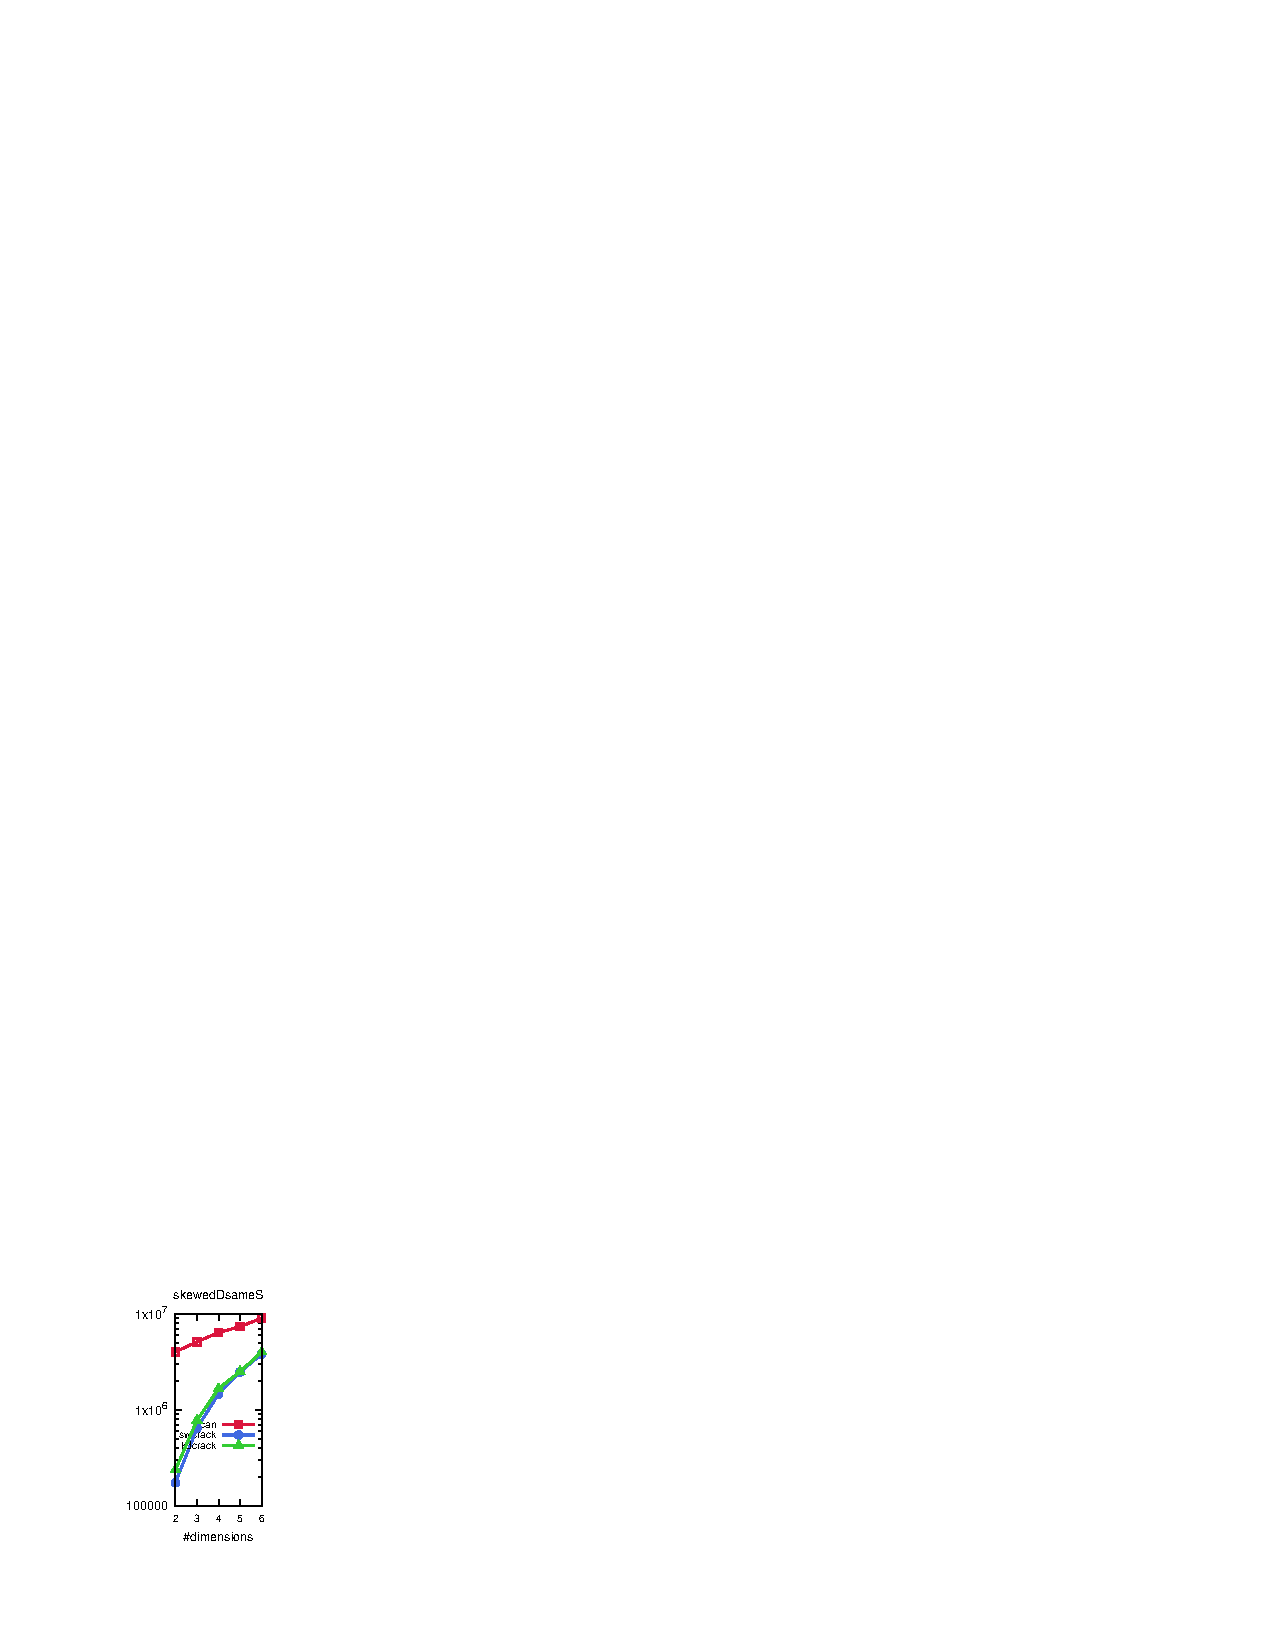
\includegraphics[trim=2.4cm 2.1cm 17cm 22cm]{Figures/vary_dimensions/skewedDsameS_vary_dimensions}
        }%
        \subfigure[]{%
            \label{fig:sequentialDsameS}
            \includegraphics[trim=2.4cm 2.1cm 17cm 22cm]{Figures/vary_dimensions/sequentialDsameS_vary_dimensions}
        }%
	\subfigure[]{%
            \label{fig:periodicalDsameS}
            \includegraphics[trim=2.4cm 2.1cm 17cm 22cm]{Figures/vary_dimensions/periodicalDsameS_vary_dimensions}
        }%
	\subfigure[]{%
            \label{fig:zoominDdifferentS}
            \includegraphics[trim=2.4cm 2.1cm 17cm 22cm]{Figures/vary_dimensions/zoominDdifferentS_vary_dimensions}
        }
    \caption{Varying $\#$dimensions of \emph{1000} queries for different workloads.}
   \label{fig:vary_dimensions}
    \end{center}
\end{figure*}


\textbf{Hardware/Software description.}

\textbf{Microbenchmark description.}

It would be nice if we included at least one experiment with real data or a standard benchmark like tpch.
Look if skyserver can be a useful example here.

\textbf{Experiments.}


\begin{figure*}[t]
     \begin{center}
        \subfigure[]{%
            \label{fig:randomDrandomS}
            \includegraphics[width=0.2\columnwidth]{Figures/kdtree/kdtree_randomDrandomS}
        }%
	\subfigure[]{%
            \label{fig:randomDsameS}
            \includegraphics[width=0.2\columnwidth]{Figures/kdtree/kdtree_randomDsameS}
        }%
        \subfigure[]{%
            \label{fig:randomDSBsameS}
            \includegraphics[width=0.2\columnwidth]{Figures/kdtree/kdtree_randomDSBsameS}
        }%
	\subfigure[]{%
            \label{fig:skewedDsameS}
            \includegraphics[width=0.2\columnwidth]{Figures/kdtree/kdtree_skewedDsameS}
        }%
        \subfigure[]{%
            \label{fig:sequentialDsameS}
            \includegraphics[width=0.2\columnwidth]{Figures/kdtree/kdtree_sequentialDsameS}
        }%
	\subfigure[]{%
            \label{fig:periodicalDsameS}
            \includegraphics[width=0.2\columnwidth]{Figures/kdtree/kdtree_periodicalDsameS}
        }%
	\subfigure[]{%
            \label{fig:zoominDdifferentS}
            \includegraphics[width=0.2\columnwidth]{Figures/kdtree/kdtree_zoominDdifferentS}
        }
    \caption{kd-tree shape after $20$ queries in different workloads.}
   \label{fig:workload}
    \end{center}
\end{figure*}


\section{Related Work}
\label{sec:related_work}

In this section we briefly discuss state-of-the-art indexing methods for handling multidimensional point data.

\textbf{Range Search in Data Points.}
One of the most basic data operations is that of filtering data that qualify a query predicate.
The query is in the form of a multidimensional range $R$ and it says ``find me the data points in the database that belong to $R$''.
The main idea in state-of-the-art multidimensional indexes is to divide the whole space into subregions \cite{Samet:book}.

 
Our work follows the same high level principles, i.e., data split, but it is the first to introduce  an adaptive indexing mechanism driven by query predicates.  
In all previous work, the index is built in one step a priori and no queries may be processed until the index is ready. 
On the contrary, in our work, query processing and index building are interleaved, resulting in a drastically reduced data to query time.






\textbf{Multidimensional Adaptive Indexing.} Even though in this paper we follow the same philosophy as in database cracking, our work is the first to design an adaptive index for multidimensional data.% processing and range search queries during query time.
Contrary to working with unidimensional arrays as in column-store relational databases in the case of database cracking, our work is based on multidimensional arrays,  which are suited for multidimensional indexing, where we index more than one columns at a time.  
Columns that are not indexed, can still be aligned using sideways cracking \cite{DBLP:conf/sigmod/IdreosKM09} which has been proposed in order to handle late tuple reconstruction in an adaptive column-store.
The concepts that have appeared in past adaptive indexing work apply here as well.
For example, updates and concurrency control can be handled exactly as in \cite{DBLP:journals/pvldb/GraefeHIKM12, CrackingTransactions, DBLP:conf/sigmod/IdreosKM07}.
Contrary to state-of-the-art multidimensional indexing work, initialization cost is kept low, bringing the ability to query the data set much sooner.   
We show both the significant bottleneck faced by state-of-the-art indexing as we grow to large data,
as well as the drastic improvement that adaptive indexing brings.

\section{Conclusions}
\label{sec:conclusions}

\textbf{Synopsis of paper focus hypothesis.}

\textbf{Synopsis of claim and results achieved.}

\textbf{Open issues for future work.}


%\scriptsize

\end{document}
